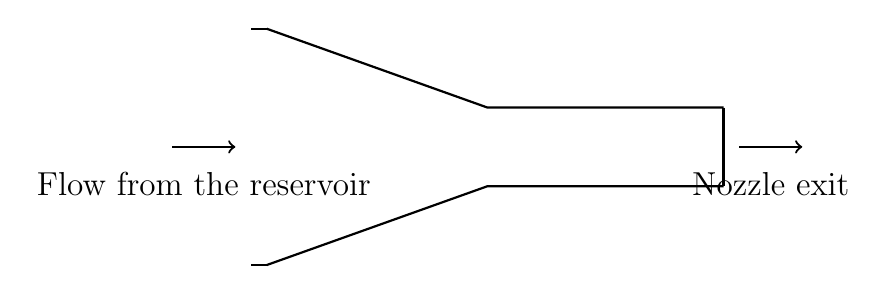
\begin{tikzpicture}
    % Draw the nozzle shape with short vertical lines at the opening
    \draw[thick] (-3,1.5) -- (-2.8,1.5);
    \draw[thick] (-3,-1.5) -- (-2.8,-1.5);
    \draw[thick] (-2.8,1.5) -- (0,0.5) -- (3,0.5);
    \draw[thick] (-2.8,-1.5) -- (0,-0.5) -- (3,-0.5);
    
    % Vertical line at the nozzle exit
    \draw[thick] (3,0.5) -- (3,-0.5);

    % Flow direction arrows
    \draw[->, thick] (-4,0) -- (-3.2,0);
    \draw[->, thick] (3.2,0) -- (4,0);

    % Labels for the flow and nozzle exit, placed below arrows
    \node[below] at (-3.6,-0.2) {\large Flow from the reservoir};
    \node[below] at (3.6,-0.2) {\large Nozzle exit};
\end{tikzpicture}
